% --- PREAMBULO (lualatex / pdflatex) ---
\documentclass[11pt, a4paper]{article}
\usepackage[a4paper, top=2.5cm, bottom=2.5cm, left=2cm, right=2cm]{geometry}
\usepackage[T1]{fontenc}
\usepackage[utf8]{inputenc}
\usepackage{lmodern}
\usepackage{amsmath}
\usepackage{array}
\usepackage{booktabs}
\usepackage{xcolor}
\usepackage{graphicx}
\graphicspath{{./}}
\usepackage{fancyhdr}
\usepackage{titlesec}
\usepackage{lastpage}
\usepackage[section]{placeins}
\usepackage[hidelinks]{hyperref}
\usepackage[spanish, es-tabla]{babel}

\usepackage{enumitem}
\setlist[itemize]{label=-}

% Paleta
\definecolor{primary}{HTML}{0F172A}
\definecolor{alertred}{HTML}{DC2626}
\definecolor{accentgreen}{HTML}{0F766E}
\definecolor{warnamber}{HTML}{D97706}
\definecolor{lightgray}{HTML}{F8FAFC}
\definecolor{darkgray}{HTML}{475569}
\definecolor{markred}{HTML}{FEE2E2}
\definecolor{markgreen}{HTML}{D1FAE5}
\definecolor{markamber}{HTML}{FEF3C7}

\newcommand{\mR}[1]{{\setlength{\fboxsep}{1.5pt}\colorbox{markred}{\textbf{#1}}}}
\newcommand{\mG}[1]{{\setlength{\fboxsep}{1.5pt}\colorbox{markgreen}{\textbf{#1}}}}
\newcommand{\mA}[1]{{\setlength{\fboxsep}{1.5pt}\colorbox{markamber}{\textbf{#1}}}}

\newcommand{\alertbox}[2]{%
  \noindent\colorbox{lightgray}{%
    \parbox{\dimexpr\textwidth-2\fboxsep\relax}{%
      \raggedright\smallskip
      \textbf{\color{alertred}{#1}}\par\smallskip
      \small #2\par\smallskip}}%
  \par\vspace{3mm}}
\newcommand{\successbox}[2]{%
  \noindent\colorbox{lightgray}{%
    \parbox{\dimexpr\textwidth-2\fboxsep\relax}{%
      \raggedright\smallskip
      \textbf{\color{accentgreen}{#1}}\par\smallskip
      \small #2\par\smallskip}}%
  \par\vspace{3mm}}
% Caja neutra para resumenes de DATOS objetivos
\newcommand{\databox}[2]{%
  \noindent\colorbox{lightgray}{%
    \parbox{\dimexpr\textwidth-2\fboxsep\relax}{%
      \raggedright\smallskip
      \textbf{\color{primary}{#1}}\par\smallskip
      \small #2\par\smallskip}}%
  \par\vspace{3mm}}

\setlength{\parindent}{0pt}
\setlength{\parskip}{6pt}

\pagestyle{fancy}
\fancyhf{}
\renewcommand{\headrulewidth}{0.4pt}
\renewcommand{\footrulewidth}{0.4pt}
\fancyhead[L]{\small\color{darkgray}\textsc{Chaco For Ever} $\bullet$ Scouting Pre-Partido}
\fancyhead[R]{\small\color{darkgray}vs San Miguel $\bullet$ Fecha 21}
\fancyfoot[L]{\footnotesize\color{darkgray}Confidencial $\bullet$ Uso interno del Cuerpo Técnico}
\fancyfoot[R]{\footnotesize\color{darkgray}Página \thepage\ de \pageref{LastPage}}

\titleformat{\section}{\normalfont\Large\bfseries\color{primary}}{\thesection}{0.6em}{}[\vspace{-2mm}\noindent{\color{accentgreen}\rule{\textwidth}{1.2pt}}]
\titlespacing*{\section}{0pt}{4mm}{4mm}
\titleformat{\subsection}{\normalfont\large\bfseries\color{darkgray}}{\thesubsection}{0.6em}{}
\titlespacing*{\subsection}{0pt}{3mm}{2mm}

\hypersetup{pdftitle={Scouting Pre-Partido - Chaco For Ever vs San Miguel},
  pdfauthor={Departamento de Big Data \& Análisis Táctico}}

\begin{document}

% --- HEADER ---
\begin{center}
  \colorbox{primary}{%
    \parbox{\dimexpr\textwidth-2\fboxsep\relax}{%
      \vspace{4mm}\centering\color{white}
      \textsc{\Large Chaco For Ever} \\ \vspace{1mm}
      \textbf{\Large SCOUTING PRE-PARTIDO} \\ \vspace{1mm}
      \small Próximo rival: San Miguel (lo recibimos de local) $\bullet$ Fecha 21 $\bullet$ Temporada 2026
      \vspace{4mm}}}
\end{center}
\vspace{3mm}

\begin{tabular}{ll}
  \textbf{Destinatarios:} & Cuerpo Técnico, Comisión Directiva \\
  \textbf{Creadores:} & Cordeiro Mariano Angel y Casco Tobias \\
  \textbf{Contacto:} & cordeiromariano17@gmail.com \\
  \textbf{Partido:} & Chaco For Ever (local) vs San Miguel (visitante) \\
  \textbf{Estado:} & Sin jugarse — análisis sobre los 20 partidos de San Miguel en 2026 \\
  \textbf{Alcance:} & Datos de la temporada 2026 (Primera Nacional) \\
\end{tabular}

\vspace{3mm}
\noindent\colorbox{lightgray}{%
  \parbox{\dimexpr\textwidth-2\fboxsep\relax}{%
    \smallskip
    \small Este informe presenta primero los \textbf{datos del rival con objetividad} (secciones 1 a 7) y deja
    \textbf{nuestra interpretación y el plan de partido para el final} (sección 8). Todo el análisis se apoya en
    los 20 partidos de San Miguel en la temporada 2026.\smallskip
  }%
}
\vspace{2mm}
\hrule
\vspace{3mm}

% ==================================================================
% BLOQUE OBJETIVO (Secciones 1-7)
% ==================================================================

% --- 1. FICHA DEL RIVAL ---
\section*{1. Quién es San Miguel}

San Miguel llega con un récord de \mA{5V - 10E - 5D} en 20 partidos (17 goles a favor, 21 en contra). El dato que lo define es el empate: \mA{10 de sus 20 partidos} terminaron igualados, la mitad. Es un equipo de mitad de tabla para abajo, sin una racha ganadora larga en todo el año.

Nos visita, así que la columna que importa es su rendimiento \textbf{de visitante}: ahí es \mR{1V - 7E - 2D}, apenas 1.0 punto por partido, con 8 goles a favor y 13 en contra. Fuera de casa gana muy poco (1 en 10) y empata casi todo (7 de 10).

En el banco tiene estabilidad: \mA{Gustavo Coleoni} dirigió prácticamente toda la temporada (19 de 20 fechas). No hubo el desorden institucional de otros rivales; es un equipo con una idea sostenida.

\databox{San Miguel en una línea}{5V-10E-5D en 20 (17 GF / 21 GC). El más empatador de la liga (50\% de empates). De visitante: 1V-7E-2D, 1.0 pts/pj. DT: Coleoni, estable todo el año. Estilo directo: 46\% de posesión, 0.86 de xG por partido, 24.6 pelotazos largos y 13.3 faltas por partido.}

\begin{figure}[htbp]
  \centering
  \fbox{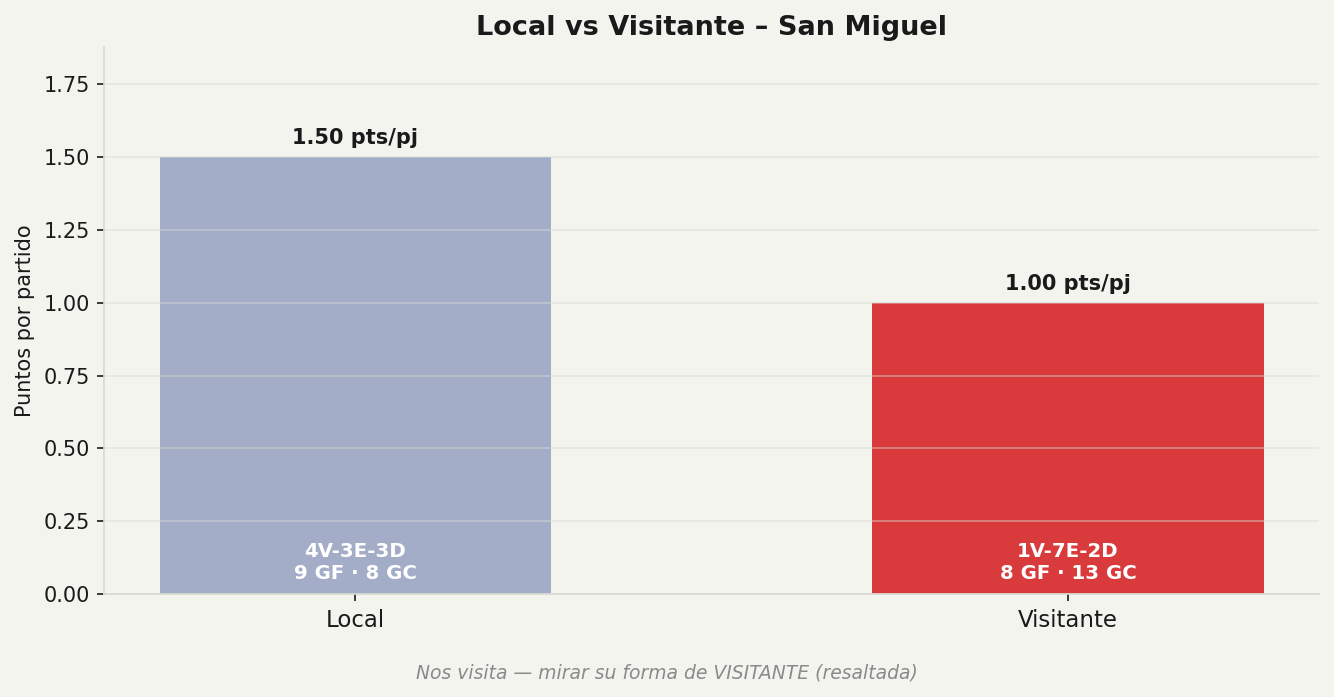
\includegraphics[width=0.58\textwidth]{local_visitante_rival.png}}
  \caption{Rendimiento de San Miguel según la cancha. La columna roja (visitante) es la que nos toca: 1.0 punto por partido, con 7 empates en 10 salidas.}
\end{figure}

% --- 2. SU EQUIPO ---
\section*{2. Su Equipo y Formación}

Su dibujo de cabecera es el \mA{4-4-2}, que usó en 17 de sus 20 partidos. En las últimas fechas probó una variante de 4-3-3 (contra Acassuso y Central Norte), pero volvió al 4-4-2 en la fecha siguiente. Es su base, con esa alternativa como plan puntual.

El once más repetido tiene al arquero como una de sus notas más altas —\mA{Lungarzo y Reynoso} se repartieron el arco y los dos promedian alrededor de 7.0—, una defensa de cuatro con \mA{Ceceri} (19 de 20 partidos, el más constante) y Cardozo como referencias, un mediocampo de cuatro (Ramírez, Ferrero, Oses, Serra) y una dupla de ataque \mA{Nasta - Delgado}. El de mejor puntería entre los de campo es el volante \mA{M. Oses} (6.99).

\begin{figure}[htbp]
  \centering
  \fbox{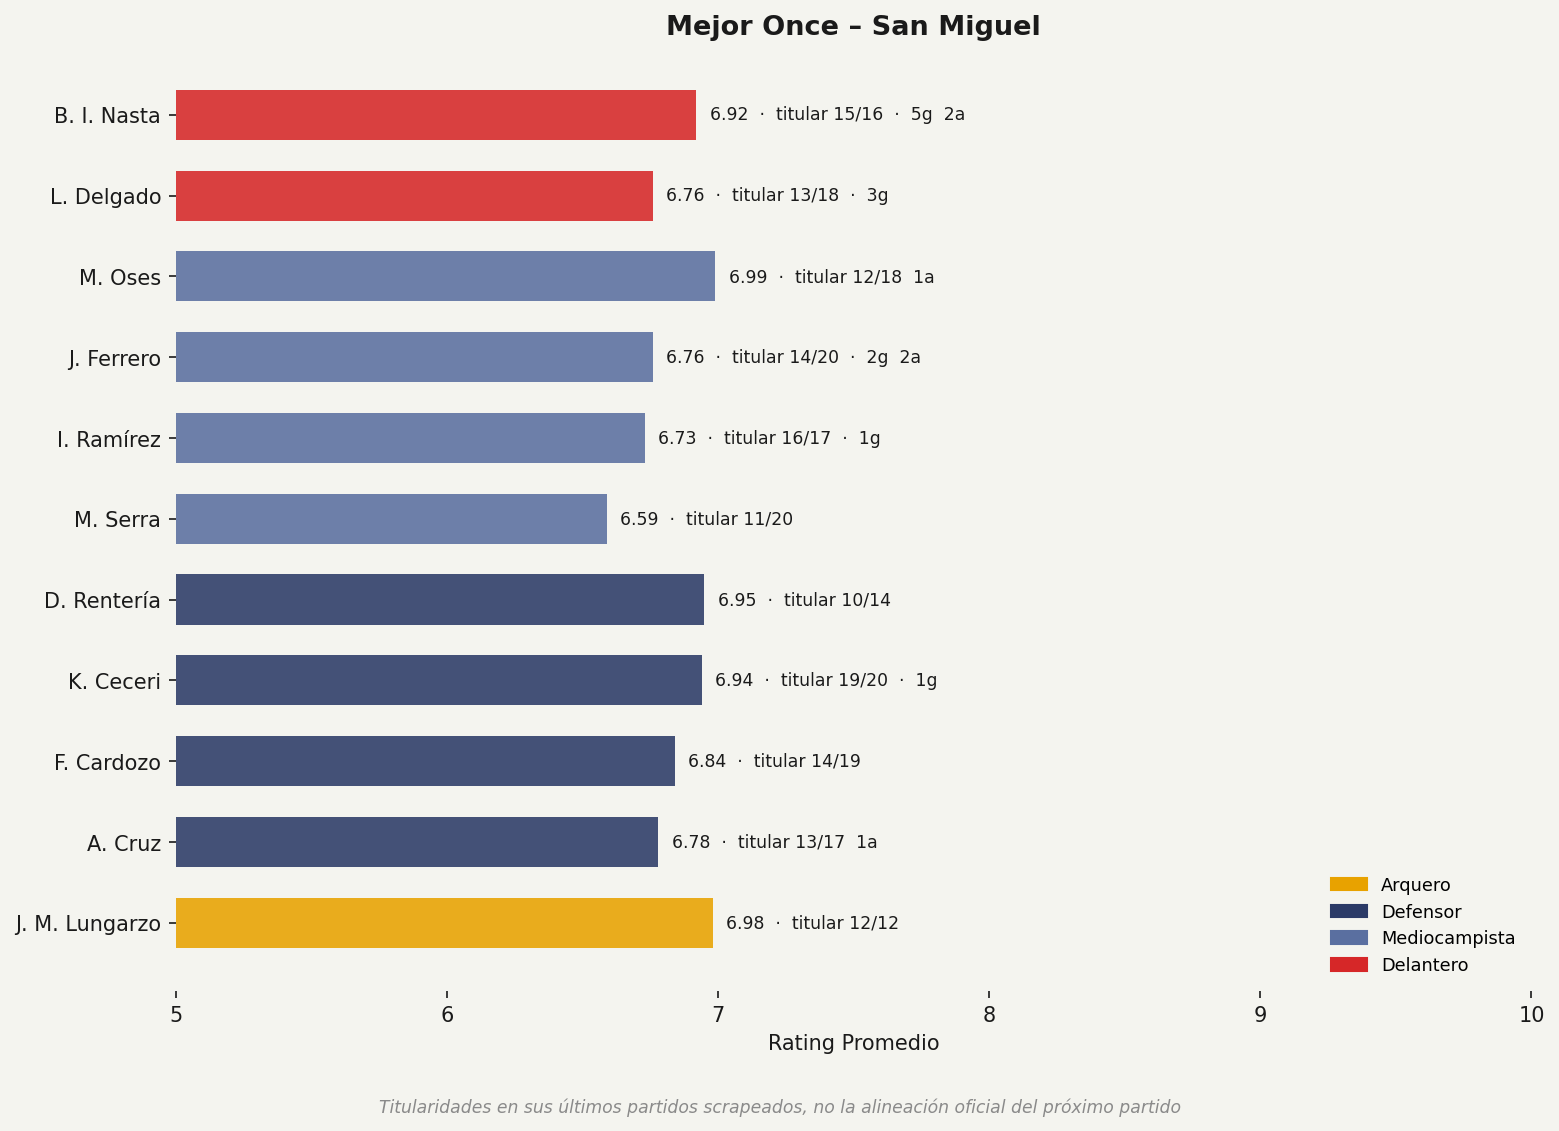
\includegraphics[width=0.62\textwidth]{mejor_once_rival.png}}
  \caption{Once más repetido de San Miguel. Nasta (5 goles) y Delgado (3) son la dupla ofensiva; Ceceri, el ancla defensiva; Oses, el mediocampista mejor puntuado.}
\end{figure}

% --- 3. COMO ATACA Y DONDE SUFRE ---
\section*{3. Cómo Ataca y Dónde Sufre}

Ofensivamente es un equipo de bajo volumen. Casi todo su peligro nace del \mA{juego abierto} (8.4 de xG y 10 goles en el año); las pelotas paradas le aportan poco. Y en ese mismo juego abierto \mR{recibe más de lo que genera} (14 goles en contra). Su grieta más marcada está en los \mR{laterales} y segundas jugadas, donde concede 3.6 de xG, bastante más de lo que produce por esa vía.

En la comparación directa, los dos equipos tienen \mA{perfiles ofensivos casi calcados} (goles 0.85 y 0.85, xG 0.87 y 0.86, remates 9.9 y 10.2). Atrás, San Miguel recibe menos goles (1.05 contra 1.30), pero Chaco concede \mG{menos xG (0.98 vs 1.04)} y menos remates (9.7 vs 10.4): parte de la diferencia de goles la explica su arquero, no un bloque más sólido. San Miguel defiende replegado, a base de despejes (20.5 por partido) e intercepciones.

\begin{figure}[htbp]
  \centering
  \fbox{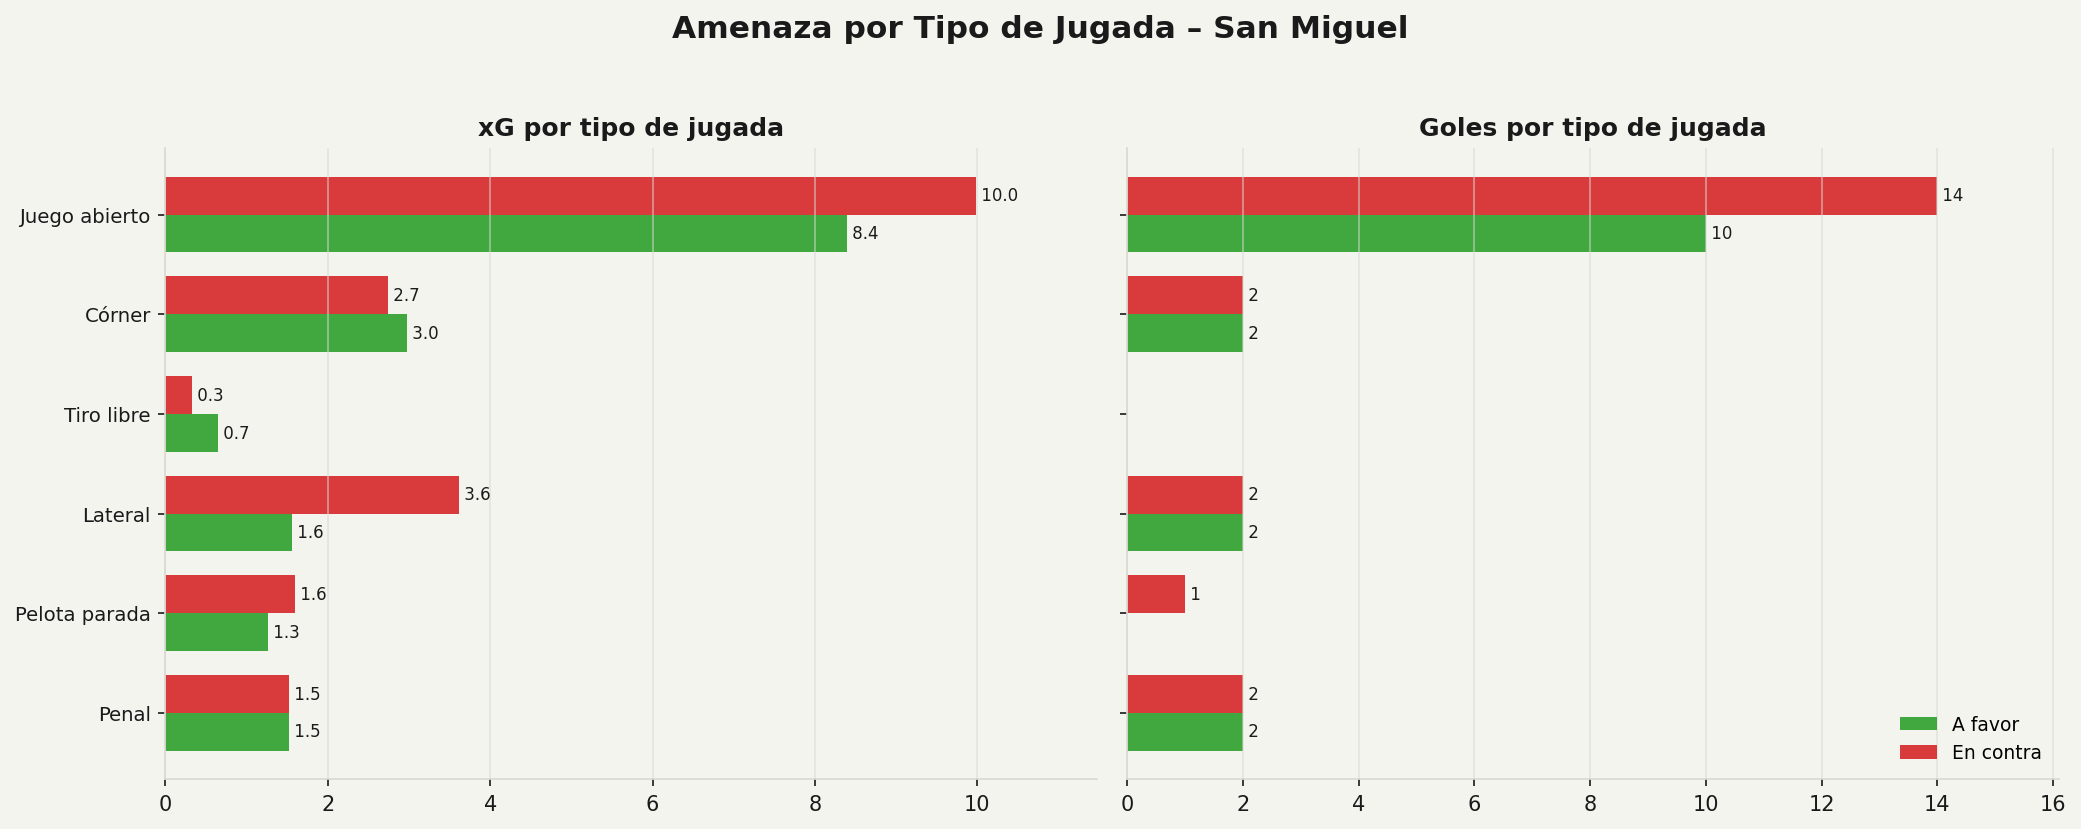
\includegraphics[width=0.82\textwidth]{amenaza_rival.png}}
  \caption{xG y goles de San Miguel por tipo de jugada. Genera poco y casi todo por juego abierto; sufre en juego abierto (14 goles en contra) y en los laterales (3.6 de xG concedido).}
\end{figure}

\subsection*{Cuándo recibe}
San Miguel concede sobre todo en las \mR{dos puntas del partido}: 6 de sus 21 goles en contra llegaron en los \mR{primeros 15 minutos} y 7 en los \mR{últimos 15}. Entre esas dos franjas suman el 62\% de los goles que recibió. En el medio del partido, en cambio, es sólido: apenas 1 gol en contra en el tramo 31-45 y 1 en el 61-75. Se lastima arrancando y cerrando, no en el desarrollo.

\begin{table}[h!]
  \centering
  \caption{Goles recibidos por San Miguel según el minuto (20 partidos)}
  \vspace{2mm}
  \begin{tabular}{lcccccc}
    \toprule
    \textbf{Franja} & \textbf{0-15} & \textbf{16-30} & \textbf{31-45} & \textbf{46-60} & \textbf{61-75} & \textbf{76-90} \\
    \midrule
    Goles en contra & \mR{6} & 3 & 1 & 3 & 1 & \mR{7} \\
    \bottomrule
  \end{tabular}
\end{table}

% --- 4. DUELOS INDIVIDUALES ---
\section*{4. Duelos Individuales}

Cruzamos a nuestros jugadores contra sus referentes. Los números por 90 minutos, sin interpretar todavía.

\begin{itemize}
  \item \textbf{Romero vs Nasta (los goleadores).} Nasta es \mA{la amenaza de San Miguel}: 5 goles, 2 asistencias y 0.436 de xG por partido, por lejos el más alto del plantel. Nasta gana en xG, tiros al arco y regates; Romero, en goles, duelos ganados, pases clave y xA.
  \item \textbf{Gaggi vs Ferrero (los volantes).} Ferrero es el mediocampista más completo de San Miguel (2 goles, 2 asistencias) y \mR{nos convirtió en la ida}. Está más volcado a lo defensivo (quites, intercepciones); Gaggi lo supera en tiros al arco, pases clave, xA y toques.
  \item \textbf{Fernández vs Adín (banda vs grieta).} Fernández es de los nuestros que más genera por afuera (pases clave, xA, regates); Adín es un central de duelo y despeje, y está \mR{a una amarilla} de la suspensión. El cruce da de lleno en la vía por la que San Miguel más sufre.
  \item \textbf{Canuto vs el arco de San Miguel.} Canuto viene de 7.8 y cinco atajadas; enfrente, San Miguel se apoya en un arco que promedia 2.6 atajadas por partido y dos porteros de nivel similar (Lungarzo / Reynoso).
\end{itemize}

\begin{figure}[htbp]
  \centering
  \fbox{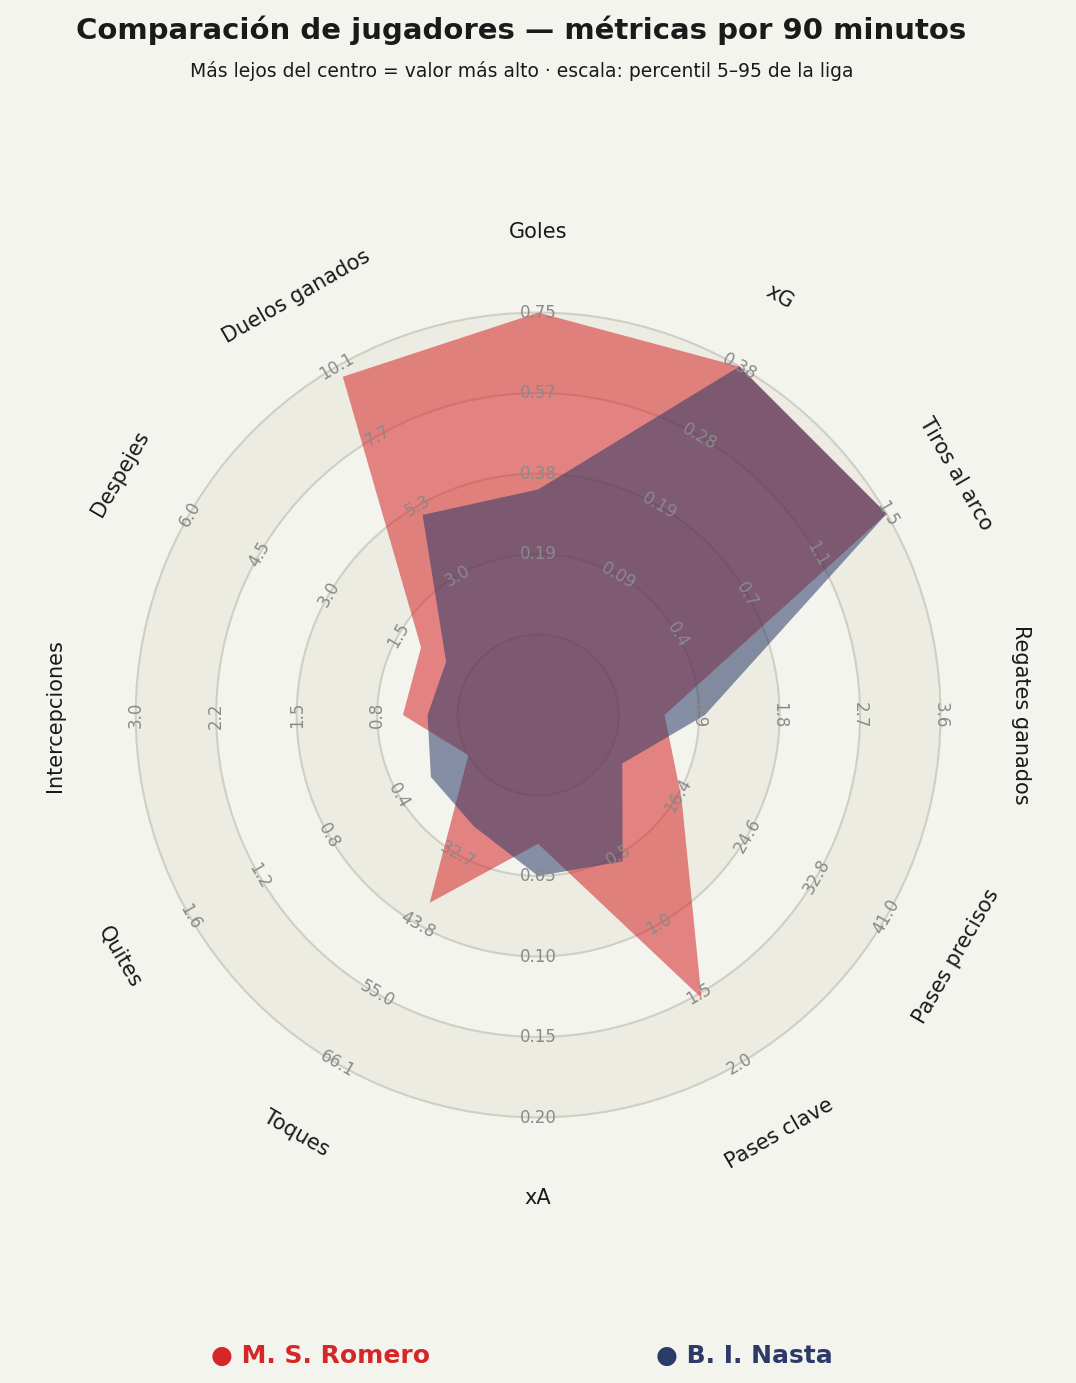
\includegraphics[width=0.52\textwidth]{Romero_vs_Nasta.png}}
  \caption{El duelo estrella: Romero (nosotros, en rojo) vs Nasta (ellos, en azul), por 90 minutos. Nasta remata y gambetea más; Romero define y asocia más. Los gráficos de Gaggi vs Ferrero y Fernández vs Adín están en la carpeta del partido.}
\end{figure}

% --- 5. DISCIPLINA ---
\section*{5. Disciplina}

San Miguel tiene \mR{tres jugadores} a una amarilla de la suspensión: D. Adín (defensor), I. Ramírez (volante) y J. Ferrero (volante). Su goleador, Nasta, es además el más indisciplinado del plantel (6 amarillas y 1 roja en 16 partidos). Es un equipo que defiende con faltas (13.3 por partido) y llega expuesto en varios nombres.

% --- 6. ULTIMO CRUCE ---
\section*{6. El Último Cruce (Ida)}

En la ida (Fecha 3, en cancha de San Miguel) perdimos \mR{2-0}, con goles de Delgado (67') y Ferrero (84'). Pero los números del partido cuentan otra cosa: Chaco \mG{generó más} (1.39 de xG contra 0.91) y remató más (14 a 12). Fue un partido que se emparejó —incluso se inclinó— para nuestro lado en juego, y se perdió por no convertir y por dos golpes puntuales de ellos.

\begin{figure}[htbp]
  \centering
  \fbox{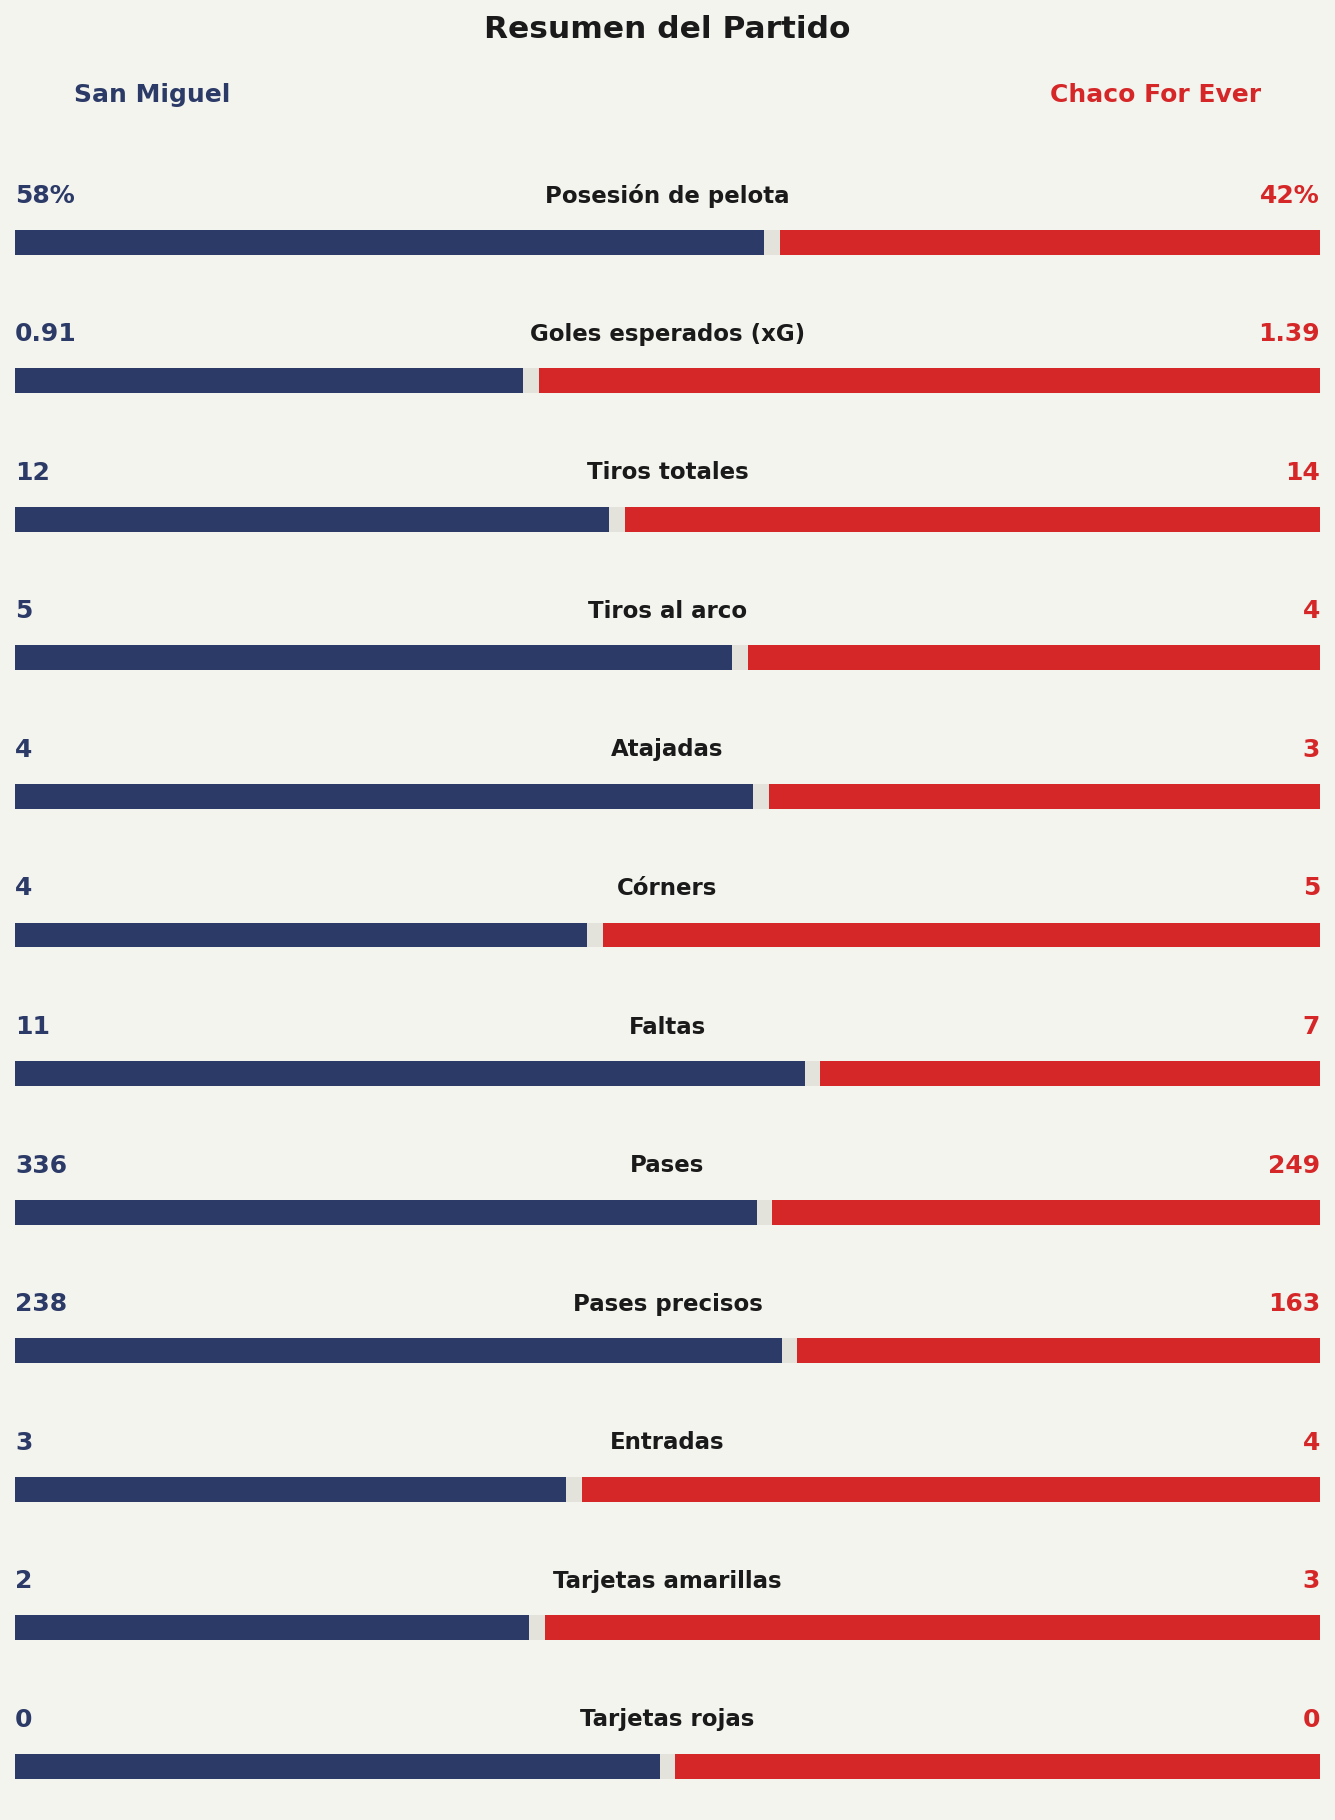
\includegraphics[width=0.66\textwidth]{ultimo_cruce_stats.png}}
  \caption{Estadísticas de la ida. Perdimos 2-0 pese a superar a San Miguel en xG y en remates.}
\end{figure}

% --- 7. MARKOV ---
\section*{7. Cómo Evoluciona el Marcador}

Modelamos con una cadena de Markov cómo se mueve el resultado de San Miguel gol a gol. Dos datos objetivos:

Primero, \mR{no cierra los partidos}: cuando se pone en ventaja por un gol, la deja escapar el 78\% de las veces (7 de 9), y 5 de esas después del minuto 70. Segundo, \mR{reacciona mal cuando le convierten}: estando un gol abajo, cae a dos abajo el 67\% de las veces y solo empata el 33\%.

% ==================================================================
% BLOQUE SUBJETIVO (Seccion 8): interpretacion y plan
% ==================================================================

% --- 8. NUESTRA LECTURA Y PLAN ---
\section*{8. Nuestra Lectura y Plan de Partido}

Hasta acá, los datos. Lo que sigue es \textbf{nuestra interpretación} y el plan que proponemos, a criterio del entrenador.

Para nosotros, San Miguel viene a buscar el empate: es el más empatador de la liga y de visitante es 1-7-2, un equipo directo, de bloque bajo, que corta con faltas y se agarra del arquero. El riesgo no es que nos ganen —afuera ganan poquísimo—, es que nos enganchen en un empate chato. La llave, otra vez, es la eficacia: en la ida los superamos en juego y perdimos igual.

\successbox{Las tres claves, a nuestro criterio}{
  1. \textbf{Paciencia y volumen para romper el bloque.} Se repliega y no presiona: da tiempo para elaborar. Insistir por su grieta —juego abierto y, sobre todo, los laterales (3.6 de xG concedido)—. \\[1mm]
  2. \textbf{Eficacia, la lección de la ida.} Generar no alcanzó la vez pasada: las claras hay que meterlas. \\[1mm]
  3. \textbf{Golpear temprano y seguir hasta el final.} Recibe casi todos sus goles en las dos puntas (6 en los primeros 15', 7 en los últimos 15') y no cierra los partidos (diluye la ventaja el 78\%). Salir a matarlo de entrada y no aflojar en el cierre: ahí es donde se rompe.
}

\alertbox{Lo que hay que cuidar}{Casi todo el peligro de San Miguel pasa por Nasta (contra y pelota parada): marca cercana y no regalarle transiciones. Ferrero llega desde el medio y ya nos convirtió en la ida. Y ojo con no regalar el partido: sin errores propios ni penales tontos, a este San Miguel le cuesta mucho lastimar. Adín, Ferrero y Ramírez, al borde de la suspensión, son presionables.}

\end{document}
